% -----------------------------------------------
% Template for SMC 2021
% Adapted from previous SMC paper templates
% -----------------------------------------------
\documentclass{article}
\usepackage{smc2021}
%%%%%%%%%%%%%%%%%%%%%%%% Some useful packages %%%%%%%%%%%%%%%%%%%%%%%%%%%%%%%
%%%%%%%%%%%%%%%%%%%%%%%% See related documentation %%%%%%%%%%%%%%%%%%%%%%%%%%
\usepackage[caption=false, font=footnotesize]{subfig}% Modern replacement for subfigure package
\usepackage{paralist}% extended list environments
\usepackage[figure,table]{hypcap}% hyperref companion
\usepackage{multirow}
% Enable for Review only, remove for Camera Ready version
\pagewiselinenumbers


% Use this if english is the only language/alphabet used in the document
\usepackage[english]{babel}


% Title.
% ------
\def\papertitle{Source separation methods for computer-assisted orchestration}

% Authors
% Please note that submissions are NOT anonymous, therefore 
% authors' names have to be VISIBLE in your manuscript. 
% Authors are entered as an ordered list, each one can be linked to multiple affiliations using the correct index.
% Available tags for authors are: \firstname \middlename \lastname \generation \originalname \email \orcid
% Available tags for affiliations are: \unit \department \institution \streetaddress \city \state \postcode \country \type
% type can take as value: University, Company, Music, Independent, Other
%
% \author[]{\mbox{\firstname{}\middlename{}\lastname{}\originalname{}\generation{}\email{}\orcid{}}}
% mbox force an author not to be split over multiple lines
\author[1]{\mbox{\firstname{Luke}\lastname{Dzwonczyk}\email{dz.luke@berkeley.edu}}}
\author[1, 2, 3]{\mbox{\firstname{L\'eo}\lastname{Ch\'edin}}}
\author[1]{\mbox{\firstname{Alejandro}\lastname{Saldarriaga-Fuertes}}}
\author[1]{\mbox{\firstname{Max}\lastname{Sherr}}}
\author[3]{\mbox{\firstname{H\'el\`ene-Camille}\lastname{Crayencour}}}
\author[1]{\mbox{\firstname{Carmine-Emanuele}\lastname{Cella}}}


%%Affiliations
\affil[1]{\department{Center for New Music and Audio Technologies}\institution{University of California, Berkeley}\city{Berkeley}\state{California}\country{USA}\affiliationtype{University}}
\affil[2]{\department{\'Ecole Normale Sup\'erieure Paris-Saclay}\institution{Universit\'e Paris-Saclay}\city{Paris}\state{}\country{France}\affiliationtype{University}}
\affil[3]{\department{Laboratoire des Signaux et Syst\`emes}\institution{Centrale Sup\'elec, CNRS, Universit\'e Paris-Saclay}\city{Paris}\state{}\country{France}\affiliationtype{University}}



% Complete setup stage
\completesetup

% Title.
% ------
\title{\papertitle}
% ***************************************** the document starts here ***************
\begin{document}
	%
	\capstartfalse
	\maketitle
	\capstarttrue
	%
	
	\begin{abstract}
		In this paper, we will study the possibility of adding source separation as a pre-processing step to the computer-assisted orchestration process. We first discuss the motivation of this addition and its potential to increase the quality of orchestrations of multi-layered sounds. Second, we select several state-of-the-art models for both music source separation (separation of instruments) and universal sound separation (separation of arbitrary sounds of different types), and compare their effectiveness for the task of orchestration. We assess which methods best suit the needs of orchestration by applying them on hand picked target sounds, orchestrating the separated outputs, and finally comparing them to the orchestration of the same target without separation. Our experiments show that the quality of orchestrations improves, both qualitatively and quantitatively, indicating that our approach is promising. Finally, we compare unsupervised methods to supervised methods for separation, and comment on the effect of training data selection on performance of supervised methods.
	\end{abstract}
	%
	
	\section{Introduction}\label{sec:introduction}
	 
	Computer-assisted composition is a field that focuses on the creation of computational tools to aid in the musical composition process \cite{FerVic2013, Ari2005}. Within this field, target-based computer-assisted musical orchestration is an example of how musical creativity can be supported by tools such as machine learning. Orchestration has been traditionally taught in an intuitive and non-formalized way, and computer-assisted orchestration seeks to help composers by accelerating certain creative processes. In particular, target-based computer-assisted orchestration helps composers explore new timbral possibilities by combining instrumental samples in such a way as to mimic the timbre of a given target sound. Formally, it is the process of creating an orchestral score that best matches an arbitrary target sound given a similarity metric and constraints~\cite{Maresz2003}.
	
	Computer-assisted orchestrations can be divided into two categories: static and dynamic. Static orchestration considers the target as a single vector of timbral features and creates a single onset of note(s) as the solution. Dynamic orchestration considers a time series of features, which allows it to create an orchestration that evolves over time with multiple onsets. It uses time segmentation to cut the target in time into multiple segments, and orchestrates each segment.
	
	Orchidea is a framework and set of tools that is currently considered the state-of-the-art for computer-assisted orchestration. It embeds the target in a feature space and uses a jointly-optimized heuristic and constraint solver to find a combination of samples that best match the target~\cite{Cella18, Cella2020}. Orchidea is able to do both static and dynamic orchestration. In order to better observe the effects of source separation, we perform only static orchestrations in this paper. The reasoning for this is that we wish to disentangle the two difficult problems of source separation and time segmentation. By only performing static orchestrations, we reduce the complexity of the problem by removing time segmentation and can better observe the effects of source separation. 

	Sound source separation is the process by which a single audio file is separated into multiple sound sources. A perfect separation is able to dissect a sound exactly into its constituent parts, in which each part is an independent sound event. Music source separation is a specific application of source separation in which the input audio is expected to be music that is comprised of a subset of instruments or sounds. For example, one music source separation method could attempt to split a song into three parts: voice, bass, and drums. Another aimed at orchestral music may try to separate the input into families of instruments: woodwinds, brass, strings, and percussion. In contrast, universal sound separation does not operate under the assumption that the input is of a musical nature, and can be applied to arbitrary sounds. In this case, the number of sources expected is specified, and the method will attempt to divide the input into the given number of sources.		
	
	Using source separation techniques as a pre-processing step has been shown to improve results in several music processing tasks. Source separation can be used to remove part of the spectrum in order to enhance the clarity of the features of interest for the task at hand. For instance, in the task of automatic chord estimation from audio, some authors have chosen to remove part of the spectrum related to percussive sounds to improve chord accuracy \cite{Reed_al2009}. Similarly some authors have investigated how beat tracking can be improved by using source separation as a pre-processing step for difficult songs with highly predominant expressive vocals \cite{ZapGom2012}. Source separation can also be applied to separate different components of the signal and work on them separately to reduce the complexity of the task. For instance, in the context of tempo detection~\cite{ChoRae2009}, the authors decompose the signal into sources to reduce rhythmic complexity, under the idea that some layers may be more rhythmically regular than the overall mix. Another example can be found in~\cite{GomAbecan2018} where harmonic/percussive and solo/accompaniment source separation techniques are investigated as a pre-processing step to improve predominant instrument recognition in jazz music.
		
	Source separation is an important addition to improve orchestration as it allows for the orchestration of more complex sounds in a way that makes sense in an orchestral context. Orchestral music often uses multiple layers, so by separating the layers of a target and individually orchestrating them, the resulting orchestration may improve. 
		
	For example, consider a target that has a continuous drone sound throughout and a melody playing above this drone. Without source separation, Orchidea would detect each note of the melody as a new onset and cut the target in time at each new note. However, this segmentation in time would also effect the drone, cutting it in time and forcing it to have a new onset each time the melody changes notes. The resulting orchestration would have multiple onsets for the drone, even though only one onset is needed at the beginning of the drone. When source separation is applied to this target, the drone and melody would be orchestrated separately. Therefore, the drone could be orchestrated by a single onset that lasts for the duration of the drone. At the same time, the melody could have as many new onsets as needed without affecting the drone. The orchestration would be greatly improved by removing the unnecessary onsets in the orchestration of the drone. Although this example is a dynamic orchestration, and we perform only static orchestrations, this paper represents a first step toward achieving dynamic orchestration with source separation.
		
	The codebase for this paper can be found at: \mbox{\url{https://github.com/dzluke/smc2021}}, and you can listen to a selection of targets and orchestrations here: \mbox{\url{https://dzluke.github.io/smc2021/}}.
		
	
	\section{Methodology}\label{sec:methodology}
	
	We compare the effectiveness of different source separation methods for the task of orchestration by applying the separation methods to various targets, orchestrating the separated output of the method, and finally comparing this to the orchestration of the target if no separation was performed (see Fig. \ref{fig:full_diagram}). Following the previous example, consider a target sound that is a combination of a low droning sound and high-pitched whistle. With separation, these two sounds would be disentangled into two separate sub-targets and each would be individually orchestrated. The separated orchestrations would then be combined to create the solution. This would then be compared to the orchestration if no separation had been performed.
	
	\begin{figure*}[t]
		\centering
			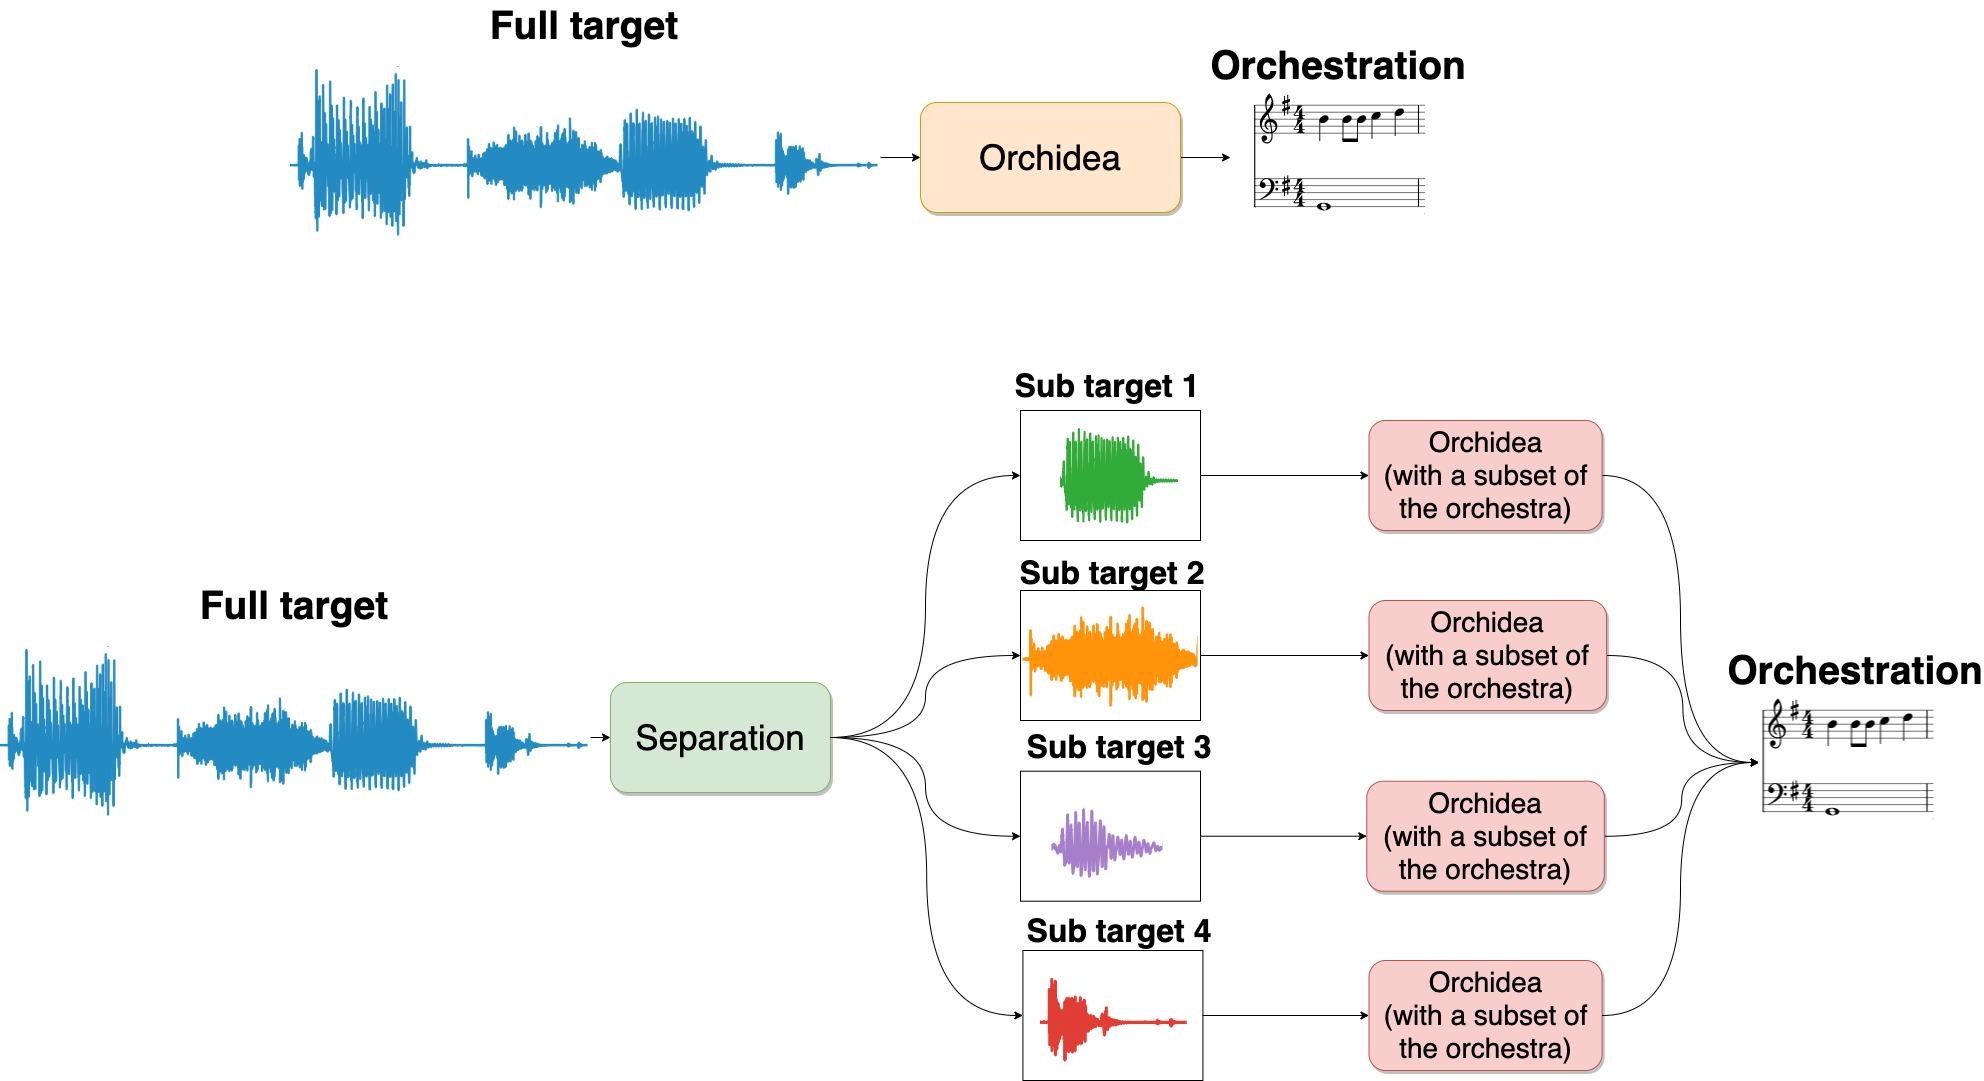
\includegraphics[width=\textwidth]{figures/diagram.png}
			\caption{Diagram comparing the process of orchestration with and without separation. At the top, the full target orchestration is created simply by orchestrating the target. At the bottom, the separation process is performed, and the resulting sub-targets are individually orchestrated with subsets of the orchestra before being recombined to obtain the full orchestration.}\label{fig:full_diagram}
	\end{figure*}
	
	
	\section{Experiments}\label{sec:experiments}
	
	We test the effectiveness of five difference source separation methods, both supervised and unsupervised, on 300 custom made targets that are combinations of sounds from different databases. During testing, a target is input to a source separation method, which outputs four sub-targets. Then each sub-target is independently orchestrated with a randomly assigned subset of the full orchestra. These orchestrations are then combined to play simultaneously, creating a final orchestrated solution. Then the distance between the target and solution is calculated, giving us a metric to compare the various separation methods. The random split of the orchestra is the same for each separation method of the same target. See Fig. \ref{fig:eval_diagram} for a diagram of this process.
	
		\subsection{Data}\label{subsec:data}
		We created our own targets as combinations of four source sounds. The sources come from the NIGENS \cite{NIGENS} and BBC \cite{BBC} databases, and freesound.org \cite{freesound}. We selected a total of 90 samples from these databases, choosing sounds that fit the following criteria: 
		
		\begin{enumerate}
			\item Static sounds that do not change harmonically over time
			\item Sounds in which there is at least some pitched content and not only noise
		\end{enumerate}			
		The sounds chosen include alarms, bells, engine noises, soundscapes, synthesizer chords, and sound effects. Each target that we used for testing was a combination of four randomly chosen source sounds from the group of 90 sounds. 
		When a target is created, the longest of the four sources is chosen to start playing at the beginning of the target. The other three sources are then randomly assigned different times to begin playing such that they will start between the beginning of the target and half-way through the longest source sound. This is done to ensure that the sources overlap and to minimize the amount of time in which there is only a single source sounding. 
		
		\subsection{Separation Methods}
	We consider source separation models trained to tackle two distinct separation problems. The first is music source separation (Open-Unmix, Demucs, ConvTasnet). For these architectures, we used models that were pre-trained on the MUSDB18 dataset~\cite{MUSDB18}. Thus, these models output 4 stereo tracks that correspond to broad instrumental categories defined in the SiSEC 2018 Mus evaluation campaign: \textit{vocals, drums, bass} and \textit{other}~\cite{Stoter_SiSEC}. It is important here to make the distinction that we did not train these models ourselves. Therefore, we cannot guarantee that the data the models were trained on is optimal for solving our problem. However, one of the goals of this paper is to explore whether pre-trained music source separation models can separate non-musical sounds in a way that improves orchestration.
	The second type of model we tested are ones that perform universal sound separation (TDCN++, NMF), which \cite{tdcnpp} defines as \textit{separating mixtures of arbitrary sounds of different types}. These methods more closely match our problem of separating non-musical target sounds.
			
			\subsubsection{Music source separation}
			\textbf{Open-Unmix}~\cite{open-unmix} is an open source implementation of a deep music source separation model, based on \cite{Uhlich2017}. It is actually composed of multiple models that are trained for each instrumental target. Each of these models is trained on the specific target using the same architecture, based on a three layer bidirectional LSTM network. Open-Unmix operates on the Short Time Fourier Transform (STFT) of the input mixture, which is first standardized. It predicts the target by multiplying the output of the LSTM network with the magnitude spectrogram of the input, essentially applying a mask. Open-Unmix also uses Wiener filtering as a last processing step.
			
			The \textbf{Demucs}~\cite{demucs} architecture is a deep learning model for musical source separation. It takes the stereo mixture as input, and outputs 4 stereo waveforms corresponding to the four categories: vocals, bass, drums and other. Demucs is based on a convolutional encoder, a bidirectional LSTM, and a convolutional decoder. The encoder and the decoder are linked with skip U-Net connections. Both the encoder and the decoder are made of 6 blocks, each made of a combination of a convolutional layer with kernel size 8, followed by ReLU activation. Finally there is another convolution with kernel size 1, followed by gated linear units (GLU). The U-network structure allows the decoder to directly access the input signal and to transfer its phase, improving results.	

			We also used the Conv-Tasnet\cite{tdcn} implementation of~\cite{demucs}, who adapted the architecture, originally designed for speech separation at 8 kHz, for the task of music source separation. Conv-Tasnet is a model based on a convolutional encoder-decoder, with a time-dilated convolutional network separation module, estimating masks based on the encoder output. This is why we refer to it as \textbf{TDCN}, in accordance with~\cite{tdcnpp}. It uses the audio waveform as input and performs a series of 1-D convolutions at different resolutions with residual connections in order to generate a pool of masks that are then applied on the embedding of the initial waveform to output the separated targets. A final 1-D convolutional layer is used as a decoder to recover the waveforms of each sub target. This type of architecture replaces RNNs in modeling sequential data, as series of dilated convolutions are a good way to capture temporal patterns.
			
			\subsubsection{Universal sound separation}
			\textbf{Non-negative matrix factorization}~\cite{Cichocki_NMF, Fevotte_NMF} is an unsupervised learning method, which takes an input non-negative matrix, in this case a spectrogram $S$, in $\mathbb{R} ^{N\times M}$ and decomposes it into a basis matrix $A$ in $\mathbb{R}^{N\times J}$ and a component matrix $X$ in $\mathbb{R}^{J\times M}$ such that $S\approx A\times X$. We use the coordinate descent algorithm from the scikit-learn Python package based on \cite{Cichocki_NMF} with $J$ set to $4$, which selects for 4 features in the dataset. We then output 4 mono waveforms containing each isolated feature $F_i$, where $F_i=A_i\times X_i$ for $i = 1, 2, 3$, or $4$.

			\textbf{TDCN++}, a version of Conv-Tasnet, was improved by \cite{tdcnpp} in order to be used for general sound separation, and not only for speech. The main architecture remains the same as in \cite{tdcn}, and the changes only affect the masking network. More specifically, feature-wise normalization replaces global normalization, residual connection ranges are extended to improve the flow of information, and learnable scale parameters are introduced to weight the outputs of each residual layer. Those modifications help the model to better extract features without drastically increasing its size.
			TDCN++ presents the interesting property of having almost the same architecture as TDCN but trained with generic sounds. Thus, it should naturally be better suited for our task, and the comparison between those two models in particular can give good insights about the impact of the data used for training.
	
		\subsection{Testing}\label{subsec:testing}
		In order to compare the effectiveness of the separation methods, a full target orchestration and a ground truth orchestration are done for each target. The \textbf{full target orchestration} is the orchestration of the target without any separation performed. The \textbf{ground truth orchestration} takes the four sources that make up the target and orchestrates each one separately, then combines the orchestrations. This ground truth represents the orchestration that could take place if the separation method was perfect and separated a target exactly into its constituent sources. 
		
		The procedure we use for testing is as follows:
		\begin{enumerate}
			\item The target is created as a combination of four randomly chosen sources, which are offset to begin playing at different times.
			\item The full target, without any separation performed, is orchestrated using the entire orchestra. This is called the full target orchestration.
			\item Each separation method is performed on the target, each splitting the target into four sub-targets. 
			\item The full orchestra is randomly split into four equal sized subsets, each containing 7 to 8 instruments.
			\item For each method, the four sub-targets are separately orchestrated, each using a different subset of the orchestra, and then each orchestration is combined to play simultaneously. This creates the \textbf{separated orchestrations}.
			\item The ground truth orchestration is created by orchestrating the four sources, using the same orchestra subsets from step 4, and then combined to play simultaneously.
			\item The distances between target and orchestration are calculated for the full target orchestration, the separated orchestration, and the ground truth orchestration. 
		\end{enumerate}	

		\begin{figure*}[t]
			\centering
				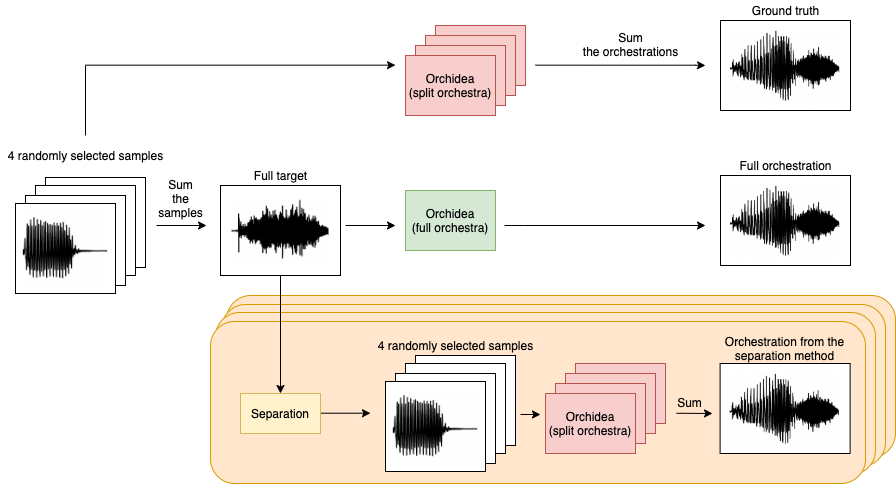
\includegraphics[width=\textwidth]{figures/evaluation_diagram.png}
				\caption{Diagram showing the testing process. Note that in both orchestrations that use a split orchestra, they use the same division of the orchestra to orchestrate their four sub-targets.}\label{fig:eval_diagram}
		\end{figure*}
		
		The orchestrations performed are static orchestrations, meaning a single onset of notes is created for each target, no matter if the target itself has multiple onsets. The OrchideaSOL database of orchestral samples is used with Orchidea to create the orchestrations~\cite{Cella2020c}. This database contains recordings of extended playing techniques, which better fits the often noisy or inharmonic nature of our targets. The full orchestra, of which non-overlapping subsets were selected to orchestrate the subtargets, contains the following instruments: 8 violins, 4 violas, 3 cellos, 1 bass, 2 oboes, 2 flutes, 2 clarinets in B$\flat$, 2 bassoons, 2 trumpets, 2 trombones, and 2 French horns.
		
		\begin{figure}[t]
		\centering
			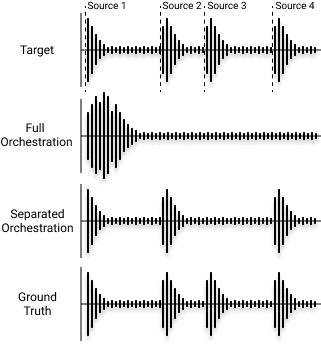
\includegraphics[width=\columnwidth]{figures/orch.jpg}
			\caption{Example waveforms showing onsets of the four sources in the target, and possible onsets in the full, separated, and ground truth orchestrations. In this example, the separation method could not distinguish between sources 2 and 3 and identified them as a single sub-target. Therefore, the separated orchestration has only 3 onsets, one of them being an orchestration that combines sources 2 and 3. Note that this is a simplified representation, in the actual targets sources overlap in time and are not as discrete as this diagram shows.}\label{fig:orchestrations}
		\end{figure}		
		
		As described in Section \ref{subsec:data}, each target is comprised of four sources that are offset in time to begin playing at different times. Figure \ref{fig:orchestrations} illustrates the effect this offset has on the full target, separated, and ground truth orchestrations. In the full target orchestration, all onsets occur at the beginning of the orchestration. Since there is no knowledge of different sources, Orchidea cannot place the different orchestrations at the appropriate offsets. For the separated orchestrations, the onsets of the sub-target orchestrations can be placed at the correct offset if the separation method has correctly separated out the sources. In the ground truth orchestration, the sources are manually offset, leading to the ground truth having each source orchestration beginning at the correct time. For this reason, despite only performing static orchestrations, the resulting separated and ground truth orchestrations are offset in time compared to the full target orchestration.
		
		\subsection{Evaluation}
		We compare the effectiveness of different separation methods by comparing how well they work for orchestration. The output of a method is orchestrated, and these orchestrations are compared. A quantitative evaluation is performed through the use of a distance metric that measures the spectral distance between target and solution. 
		
		The distance metric cuts the target and solution into successive frames that are 4,000 samples in length, which is approximately 90 milliseconds at a sampling rate of 44.1 kHz. The spectral distance, as defined in Eqn. \ref{eqn:distance}, is calculated between corresponding frames of the target and solution. The spectral distance metric is proposed in \cite{Cella2020} as part of the cost function used in Orchidea during the optimization, and used in \cite{Cella2020b} to compare accuracies of orchestrations. The equation takes in the magnitude spectrums of the FFTs of the target $x$ and of the solution $\tilde{x}$. Then for each bin $k$ of these spectrums, it calculates the absolute difference between the values. The differing values of $\lambda_1$ and $\lambda_2$ allow the metric to penalize the solution in different ways. For our purposes, we used $\lambda_1 = 0.5$ and $\lambda_2 = 10$, which penalizes a solution that overshoots the harmonic energy of the target.
		
		\begin{equation}\label{eqn:distance}
d(x, \tilde{x}) =\lambda_1 \sum_k \delta_{k1}(x_k - \tilde{x}_k) + \lambda_2 \sum_k \delta_{k2}|x_k - \tilde{x	}_k| \\
\end{equation}
where $\delta_{k1} = 1 \text{  if  } x_k \ge \tilde{x}_k, 0 \text{  otherwise}$; and $\delta_{k2} = 1 \text{  if  } x_k < \tilde{x}_k, 0 \text{  otherwise}$.
	
	
	\begin{table}[t]
		\begin{center}
			\begin{tabular}{|c|c|}
				\hline
				& Average distance \\
				\hline
				Demucs & 25.11 \\
				\hline
				Open-Unmix & 24.48\\
				\hline
				TDCN & 26.44\\
				\hline
				NMF & 22.44 \\
				\hline
				TDCN++ & 24.38 \\
				\hline
				Full target orchestration & 24.96 \\
				\hline
				Ground truth orchestration & 24.19 \\
				\hline
			\end{tabular}
		\end{center}
		\caption{Average across 300 targets showing the distance between target and orchestration for various methods. For Demucs, Open-Unmix, TDCN, NMF, and TDCN++, the value shown is the average distance between the target sound and the ``separated orchestration'' created from the output of the given separation method (see Sec. \ref{subsec:testing}). Similarly, ``Full target orchestration'' and ``Ground truth orchestration'', as defined in Sec. \ref{subsec:testing}, are the average values between target and orchestrated solution. Lower values are better.}
		\label{tab:distances}
	\end{table}
	
%	\begin{table}[t]
%		\begin{center}
%		\begin{tabular}{|c|c|c|c|}
%			\hline
%			& Model & Average distance & Variance\\
%			\hline
%			\multirow{3}{4em}{Music source separation} & Open-Unmix & 24.48 & \\
%			& Demucs & 25.11 & \\
%			& TDCN & 26.44 & \\
%			\hline
%			\multirow{2}{4em}{Universal separation} & NMF & 22.44 & \\
%			& TDCN+++ & 24.38 & \\
%			\hline
%			\multirow{2}{4em}{} & Full target & 24.96 & \\
%			\hline
%			& Ground truth & 24.19 & \\
%			\hline
%		\end{tabular}
%		\end{center}
%		\caption{Average across 300 targets showing the distance between target and orchestration for various methods. ``Full target'' means no separation was performed. Lower values are better.}
%		\label{tab:test}
%	\end{table}
	
%	\begin{figure}[t]
%		\centering
%			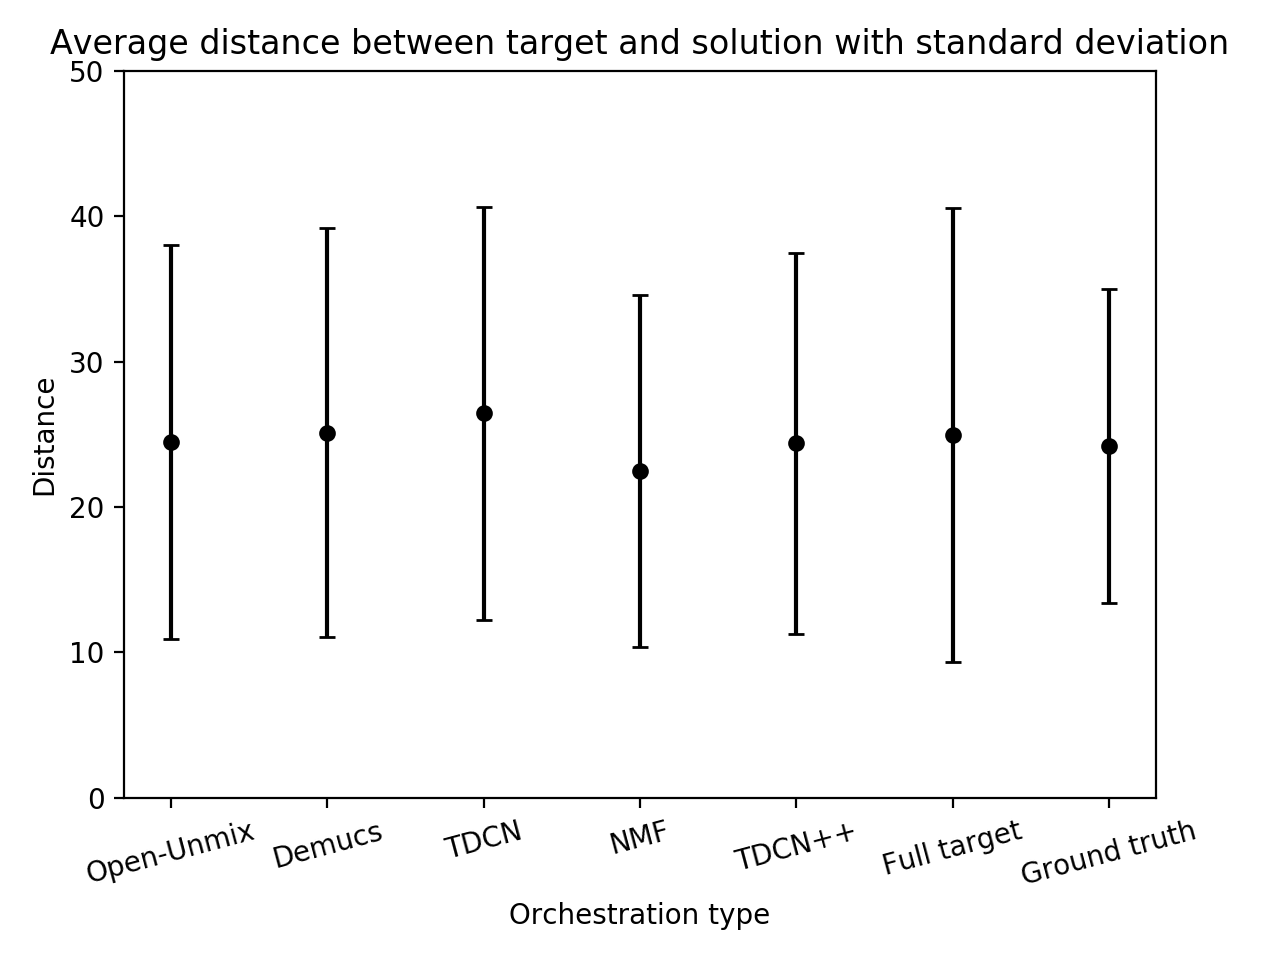
\includegraphics[width=\columnwidth]{figures/graph.png}
%			\caption{Plot showing the average distance and standard deviation between target and solution for each orchestration method.}\label{fig:plot}
%	\end{figure}
	
		\subsection{Results}
		The average distances for full target, separated, and ground truth orchestrations are displayed in Table \ref{tab:distances}. These results are the average distance between target and orchestration for 300 different targets. We found that NMF performed the best out of all separation methods, and even outperformed the ground truth orchestrations, on average. TDCN++, Open-Unmix, and NMF performed better than the full target orchestrations, meaning that separating targets using these methods leads to a better orchestration than if no separation is applied.
	
	\section{Discussion}\label{sec:discussion}
	In this paper, we addressed the problem of using source separation as a pre-processing step for computer-assisted orchestration. The results show that performing source separation followed by a static orchestration of each individual sub-target improved the spectral distance between the original target and its orchestrated version in three out of five of the methods tested. This shows that source separation is a useful pre-processing stage for computer-assisted orchestration. 
	
	Furthermore, the one unsupervised method we tested, NMF, outperformed all the supervised methods. This suggests that methods like NMF can still be useful for specific problems when available data is limited. It is logical that unsupervised methods will perform well for problems in which there is limited data, as they require less data than supervised methods. NMF also outperformed the ground truth orchestrations, which could be due to the relative simplicity of NMF's output subtargets making subsequent orchestration easier for Orchidea, but more experimentation would need to be done in order to confirm this. It is important to notice that for the supervised methods, we used pre-trained versions of the neural models. All of these models, except for TDCN++, were trained on musical data. However, we tested them on a wide range of targets, many of which were not strictly musical. This could explain why Demucs, Open-Unmix, and TDCN performed worse than NMF, and why TDCN++, which was trained on arbitrary sounds, outperformed the other supervised methods. Therefore, we may infer from our results that models trained on generic sounds generate a better separation for orchestration when compared to models trained only on musical sounds.
	
	Since unsupervised methods perform well, it is reasonable to think that supervised methods trained on a dataset of arbitrary sounds could yield better overall performance for orchestration.
	
		\subsection{Future Work}\label{sec:futurework}	
		As we stated previously, we believe that one of the reasons the supervised methods did not perform as well is because of the data they were trained on. Therefore, a natural next step is to train these models with sounds that are more appropriate for computer-assisted orchestration.
		
		Another aspect we would like to work on is the assignment of the orchestras. Currently, the subset of the orchestra that is assigned to each sub-target is randomly selected. However, it is possible that this random assignment could reduce the quality of the final orchestration. If, for example, one of the sub-targets contains mostly low pitch content, but the orchestra assigned to it contains mostly violins, violas, flutes, and oboes, the resulting orchestration will suffer. To solve this problem, a step could be added that jointly-optimizes the orchestras assigned to each sub-target, ultimately choosing an assignment that leads to the best orchestration of each sub-target.
		
		As we stated in Section \ref{sec:introduction}, we chose static orchestration instead of dynamic orchestration to avoid entangling the problems of time segmentation and source separation. Future work could include applying source separation to dynamic targets and performing dynamic orchestration.
		
		Finally, one or multiple of the separation methods we tested should be implemented in Orchidea in order to improve the orchestrations Orchidea is capable of creating. 
	
	%%%%%%%%%%%%%%%%%%%%%%%%%%%%%%%%%%%%%%%%%%%%%%%%%%%%%%%%%%%%%%%%%%%%%%%%%%%%%
	%bibliography here
	\bibliography{references}
	
\end{document}
